\chapter{Development}
\label{ch:dev}

\section{Package layout}

\begin{lstlisting}
<pkg>/
  <pkg>/
    __init__.py
    <name>_node.py        thin ROS nodes: parameters, pubs/subs, services, timers, conversions
    core/                 pure Python + numpy: algorithms, models, state machines, configs
      config.py           configuration dataclasses (dharma_utils.config.param)
      <topic>/            sub-packages for families (controllers/, avoidance/, follower/ ...)
    utils/                ROS-side helpers of this package: msg <-> core conversions, markers
  config/<pkg>.yaml       defaults (only what differs from the dataclass defaults, plus docs)
  launch/<pkg>.launch.py
  test/unit/test_*.py     pytest on core/ without ROS
  test/ros/test_*.py      rclpy in-process node tests
  test/test_style.py      dharma_utils.testing.check_package
  package.xml  setup.py  setup.cfg  resource/<pkg>  README.md  CHANGELOG.md
\end{lstlisting}

\begin{itemize}
  \item \code{core/} never imports \code{rclpy}, ROS messages, tf2 or launch; nodes convert messages
    to core types (numpy arrays, \code{Pose2D}, dataclasses) at the edge.
  \item Modules have at most 300 lines (tests 400), one class per algorithm. Families are OOP: an
    abstract base class in \code{base.py}, one implementation per file, a
    \code{dharma_utils.plugins.Registry} in \code{__init__.py}, open to entry points so a product
    adds an implementation without forking.
  \item Nodes subclass \code{dharma_utils.ros.DharmaNode} and start with \code{run(MyNode)}:
    \code{declare_config}, \code{declare_robot}, \code{self.log}, \code{self.tf} (with per-edge
    ages), \code{self.every()} (exception-guarded timers), shutdown hooks.
  \item \code{setup.py} uses \code{find_packages(exclude=['test','test.*'])} and
    \code{extras_require}\texttt{=\{'test': ['pytest']\}}: without a pytest test dependency colcon runs no
    tests and Jazzy CI fails with exit code~5.
\end{itemize}

\section{Adding a plugin}

A product adds a controller or an avoidance policy without forking \pkg{dharma_navigation}:
subclass \code{PathController} or \code{AvoidancePolicy} with a \code{Config} dataclass, and
register it under the entry point group \code{dharma.controllers} or \code{dharma.avoidance} in its
\code{setup.py}. Its parameters appear as \code{<name>.*} on the node and are validated like every
other parameter.
\todo{a complete minimal example package (phase 2)}

\section{Code style}

\begin{itemize}
  \item English, clean, readable; one-line docstrings on public classes and functions; comments
    only where the code cannot say it. No commented-out code, no \code{print}, no bare
    \code{except}.
  \item Type hints on public functions; frozen dataclasses for data and configuration; \code{Enum}
    for states; no mutable default arguments.
  \item Units in names or docstrings (\code{_sec}, \code{_m}, \code{_deg}); radians internally.
  \item Python 3.10 and numpy 1.21 compatible (Humble): no \code{typing.Self}, \code{tomllib},
    \code{StrEnum}, \code{datetime.UTC}, PEP~695, same-quote nested f-strings or numpy 2 APIs.
  \item Short functions: ruff's pylint rules (branches, statements, complexity 12) are on; split
    instead of adding \code{noqa}.
\end{itemize}

\section{Lint and format}

The same pre-commit hooks run locally and in CI: whitespace and end-of-file fixes, YAML and XML
checks, large-file guard, \texttt{ruff check --fix} and \texttt{ruff format} (single quotes, line
length 99), \code{clang-format} for C++, \code{prettier} for YAML, Markdown and JSON,
\code{shellcheck}.
\begin{lstlisting}
pip install pre-commit && pre-commit install
pre-commit run --all-files
\end{lstlisting}

\section{Tests}

\begin{description}
  \item[\code{test/unit}] pytest on \code{core/}, fast and without ROS:
    \texttt{PYTHONPATH=\$PWD python -m pytest -q test/unit}.
  \item[\code{test/ros}] rclpy in-process node tests with \code{DharmaNode}, \code{Spinner} and
    \code{Collector} (\code{dharma_utils.testing}); unique node names; \code{rclpy.init()} and
    \code{try_shutdown()} per test. Module-level helpers must not be named \code{setup} or
    \code{teardown}: the pytest versions of the Humble and Jazzy apt packages run them as nose-style
    fixtures before \code{rclpy.init()}.
  \item[\code{test/test_style.py}] \code{check_package}: module sizes, pure \code{core/}, no
    shadowed node members.
\end{description}
Every fixed defect has a regression test (Appendix~\ref{app:trace}).
\begin{lstlisting}
colcon build --packages-select <pkg>
colcon test --packages-select <pkg> --event-handlers console_direct+
colcon test-result --verbose
\end{lstlisting}

\section{Continuous integration}

\begin{figure}[h]
  \centering
  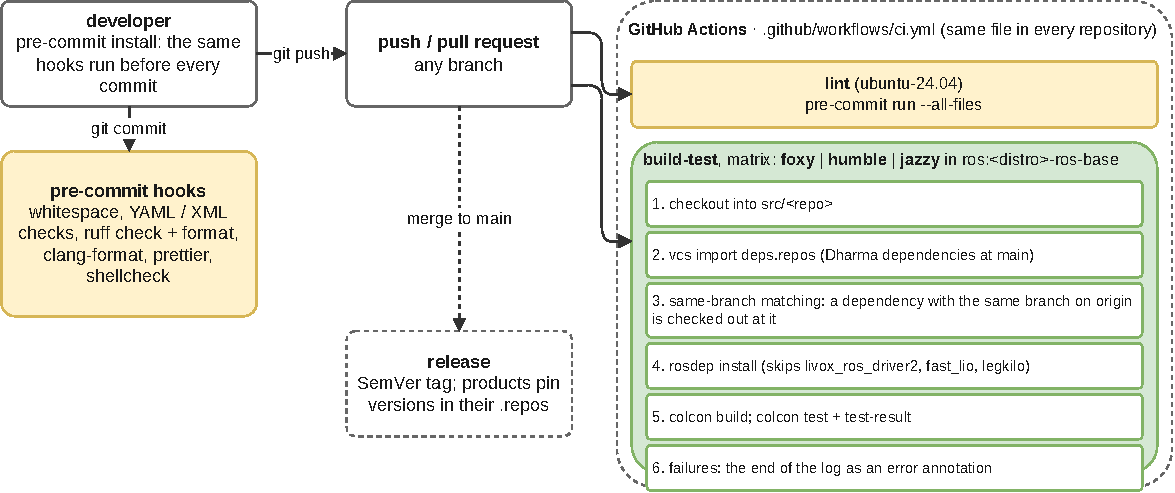
\includegraphics[width=\textwidth]{ci}
  \caption{CI of every Dharma repository: lint, then build and test on Humble and Jazzy with the
    Dharma dependencies on the same branch when it exists.}
  \label{fig:ci}
\end{figure}

Every repository carries the same \code{.github/workflows/ci.yml} (Fig.~\ref{fig:ci}):
\begin{enumerate}
  \item \textbf{lint} on Ubuntu 24.04: \texttt{pre-commit run --all-files}; the end of the log is
    reported as an error annotation on failure.
  \item \textbf{build-test}, matrix \code{humble} and \code{jazzy} in \code{ros:<distro>-ros-base}
    (Python 3.10 with numpy 1.21, and Python 3.12 with numpy 1.26):
    \begin{enumerate}
      \item check out the repository into \code{src/<repo>};
      \item \texttt{vcs import} the Dharma dependencies from \code{deps.repos} (at \code{main});
      \item \textbf{same-branch matching}: every dependency that has the branch under test on
        its origin is checked out at that branch, so a change spanning several repositories is
        built and tested together before it is merged;
      \item \texttt{rosdep install} (skipping \code{livox_ros_driver2}, \code{fast_lio},
        \code{legkilo}, which are built from source on robots);
      \item \texttt{colcon build}, then \texttt{colcon test} of the repository's packages and
        \texttt{colcon test-result}.
    \end{enumerate}
\end{enumerate}
Discovery is limited to localhost in CI (\code{ROS_LOCALHOST_ONLY}, \code{ROS_AUTOMATIC_DISCOVERY_RANGE}).

\section{Releases}

\begin{itemize}
  \item SemVer; before 1.0 a breaking change bumps the minor version and every package of the stack
    moves with it (0.1 $\to$ 0.2). \code{dharma_utils} is a dependency of every package: its API is
    deprecated one minor release before anything is removed.
  \item \code{CHANGELOG.md} in Keep a Changelog format (Added, Changed, Fixed, Removed);
    \code{package.xml} carries the version.
  \item Conventional commits, one short line each (\texttt{fix(mux): rotation inside the field}).
  \item Products pin released versions in their \code{.repos} file (vcstool).
\end{itemize}

\section{The template repository}

The \code{Dharma} repository is the hub of the stack and a GitHub template. It holds
\code{dharma.repos} (every Dharma repository at \code{main}), \code{external.repos}
(\code{livox_ros_driver2}, FAST-LIO, optionally the Leg-KILO fork), a Docker development
environment for Humble and Jazzy (desktop over VNC and noVNC), \code{scripts/dev.sh} and
\code{scripts/setup.sh}, the canonical tooling files, the placeholder bringup package
\code{robot_bringup} (robot profile, stack overrides, \code{robot.launch.py} composing the package
launch files, \code{sim.launch.py} with the simulator) and this documentation. A new product is
created with ``Use this template'' and \texttt{scripts/init\_project.py --name <Repo> --package
<bringup> --robot-ns <ns>}. \todo{verify against the finished template repository (phase 2)}

\section{Building this documentation}

\begin{lstlisting}
make -C docs              # diagrams (when draw.io is installed), manual, paper
make -C docs diagrams     # diagrams/*.drawio -> diagrams/pdf (cropped), diagrams/svg
make -C docs manual       # build/manual/dharma_manual.pdf
make -C docs paper        # build/paper/dharma.pdf
make -C docs reference SRC=~/ws/src   # regenerate manual/generated from the sources
\end{lstlisting}
Diagrams are draw.io files (Helvetica; colours per layer: estimation orange \texttt{\#ffe6cc} /
\texttt{\#d79b00}, world model blue \texttt{\#dae8fc} / \texttt{\#6c8ebf}, planning and execution green
\texttt{\#d5e8d4} / \texttt{\#82b366}, safety red \texttt{\#f8cecc} / \texttt{\#b85450}, utilities yellow
\texttt{\#fff2cc} / \texttt{\#d6b656}, hardware grey \texttt{\#f5f5f5} / \texttt{\#666666}). Their PDF and SVG
exports are committed, so LaTeX builds without draw.io.
